\documentclass[11pt,a4paper]{report}
\usepackage[utf8]{inputenc}
\usepackage[french]{babel}
\usepackage[T1]{fontenc}
\usepackage{amsmath}
\usepackage{amsfonts}
\usepackage{amssymb}
\usepackage{xcolor}
\usepackage{gensymb}

\usepackage{geometry}
\geometry{hmargin=2.5cm,vmargin=1.5cm}
\usepackage{wasysym}
\usepackage{graphicx}

\author{Mathieu Sarrat}
\title{LC9 - Molécules de la santé}

\makeatletter
\renewcommand{\thesection}{\@arabic\c@section}
\makeatother


\begin{document}
\maketitle

\section*{Niveau, Pré-requis et objectifs}
\begin{itemize}
	\item \textbf{Niveau :} Première STL-SPCL\\
	
	\item \textbf{Pré-requis :}
	\begin{itemize}
		\item Notions de stéréoisomérie,
		\item Réaction d’estérification,
		\item Réaction acido-basique,
		\item Lecture de spectres IR et RMN.\\
	\end{itemize}
	
	\item \textbf{Objectifs :}
	\begin{itemize}
		\item Définir un médicament, un principe actif, un excipient. Antiseptiques, désinfectants. 				Médicament ou poison, question de dosage.\\
		\item Appliquer les notions de synthèse organique vues au lycée pour synthétiser, purifier 
		et caractériser une molécule de la santé, l'acide acétylsalicique.\\ 
	\end{itemize}
		
	\item \textbf{Recommandations :}
	\begin{itemize}
	\item 1$\degree$) Allumer le banc Köfler
	\item 2$\degree$) Synthèse de l'aspirine complète.
	\item 3$\degree$) Pendant ce temps et juste après, préparer le dosage de la bétadine.
	\item 4$\degree$) Relancer la synthèse de l'aspirine environ 30 minutes avant l'arrivée du jury.
	\end{itemize}
\end{itemize}

\newpage
\section*{Introduction}

L'être humain a toujours cherché à survivre à son environnement, à s'adapter. Pendant longtemps, de nombreuses maladies étaient synonymes de décès à plus ou moins court terme. Lors du siècle dernier, l'espérance de vie a bondi de 48 ans à 79 ans (en 2000). Les progrès en matière de santé, permis notamment par ceux de la chimie, sont en partie responsables de cette amélioration.\\

Chimistes et biologistes se sont en effet lancés dans le vaste chantier de la compréhension du corps humain et de ses interactions avec son environnement et notamment avec les nombreux micro-organismes avec qui il cohabite. Le corps humain est de plus un véritable milieu réactionnel "sur pattes", synthétisant jour après jour de nombreuses espèces chimiques indispensable à sa survie.\\

\textbf{Par l'expérience d'abord}, essentiellement en ingérant des plantes et en remarquant leurs propriétés curatives, l'Homme a \textbf{identifié puis synthétisé} des substances capables de le soigner : on citera par exemple \textbf{la quinine}, (extraite du quinquina, un arbuste d'Amérique du Sud), utilisée pour traiter les fièvres et le paludisme, ou encore \textbf{la salicyline}, présente dans les décoctions d'écorce de saule utilisées dès l'Antiquité pour lutter contre douleurs et fièvre.\\

\begin{figure}[h!]
	\begin{center}
		\begin{tabular}{cc}
  		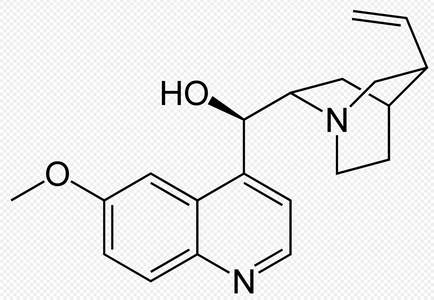
\includegraphics[scale = 0.7]{quinine.png} &
   		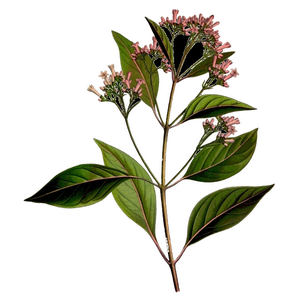
\includegraphics[scale = 0.7]{quinquina.png}\\
   		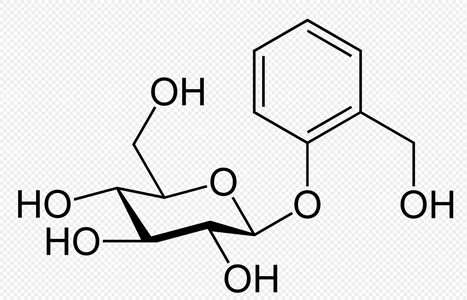
\includegraphics[scale = 0.7]{salicyline.png} &
   		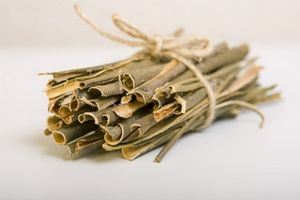
\includegraphics[scale = 0.7]{saule.png}\\
	\end{tabular}
	\caption{En haut, quinine et quinquina. En bas, salicyline et écorce de saule.}
	\end{center}
\end{figure}

Les médecins du $\text{XVIII}^\text{e}$ avaient d'ailleurs remarqué un goût similaire entre la poudre de quinquina et les décoctions d'écorce de saule, et en avaient déduit que s'ils avaient le même goût ils pouvaient tout aussi bien avoir les mêmes propriétés thérapeutiques.\\

Une fois les médicaments synthétisés, il faut s'assurer qu'ils soient propres à la consommation, avec un rapport favorable entre effets bénéfiques et effets secondaires indésirables. 

\newpage
\section{Les molécules de la santé}\label{sec:1}

On peut distinguer plusieurs catégories de molécules de la santé : par exemple les \textbf{molécules du vivant} qui constituent le corps humain (acides aminés, protéines ...), et le \textbf{médicaments} qui correspondent aux molécules interagissant avec notre organisme via des fonctions spécifiques et un mode d'action particulier, à visée thérapeutique. Dans cette leçon, on s'intéressera aux médicaments.\\

\subsection{Lien entre structure et propriétés}

Les propriétés d'une molécule découlent des fonctions chimiques qu'elle porte, de son squelette et de sa topologie. On citera par exemple la \textbf{thalidomide}, molécule possédant deux énantiomères :
\begin{itemize}
	\item la R-Thalidomide, un sédatif, utilisé notamment pour calmer les nausées des femmes enceintes,
	\item la S-Thalidomide, un composé dangereux car tératogène, c'est à dire susceptible de provoquer des malformations chez les nouveaux-nés.
\end{itemize}

\begin{figure}[h!]
	\begin{center}
  		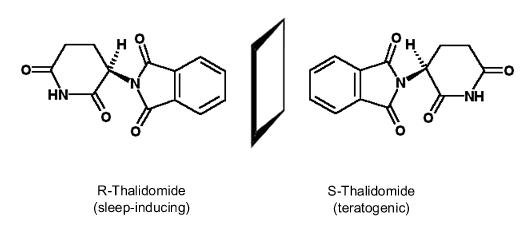
\includegraphics[scale = 0.8]{thalidomide.png}
	\caption{Énantiomères de la thalidomide.}
	\end{center}
\end{figure}

Pour l'ibuprofène, l'énantiomère S a des propriétés antalgiques, alors que l'énantiomère R n'a pas d'action (inactif, mais heureusement non toxique). On synthétise l'ibuprofène sous forme racémique (mélange 50/50 des deux énantiomères) car il est coûteux d'obtenir un énantiomère pur. Cela reste néanmoins du gaspillage de réactifs.\\

\begin{figure}[h!]
	\begin{center}
  		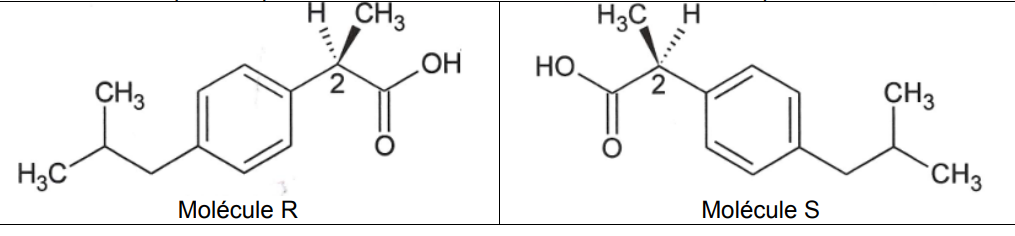
\includegraphics[scale = 0.5]{ibuprofene.png}
	\caption{Énantiomères de l'ibuprofène.}
	\end{center}
\end{figure}

\textbf{Remarque importante :} les dénominations R et S ne semblent pas au programme, mais l'énantiomérie oui...

\newpage
\subsection{Les médicaments}

\textbf{Définition :} un médicament est une substance ou composition présentant des propriétés curatives ou préventives à l'égard de maladies. Il s'agît d'un mélange de composés naturels et/ou synthétisés par l'Homme, disponible parfois sous plusieurs \textbf{formes galéniques} (gélules, comprimés, suspension, solution).\\ 

Un médicament contient un ou plusieurs principes actifs et un ou plusieurs excipients :
\begin{itemize}
	\item \textbf{principe actif :} substance active ayant un effet thérapeutique, comme le paracétamol pour le Doliprane ou l'acide acétylsalicylique pour l'Aspirine;
	\item \textbf{excipient :} substance inerte sur le plan pharmacologique servant à produire la forme galénique du médicament (liant, diluant, aromatisant ou colorant). C'est par exemple le cas de 	l'eau dans un sirop.
\end{itemize}

La \textbf{formulation} du médicament, reprend la liste des principes actifs et des excipients. Dans le cas de l'Aspirine, on peut la trouver sous \textbf{forme effervescente} : les excipients sont essentiellement l'acide citrique et l'hydrogénocarbonate de sodium. Lorsqu'on introduit un cachet dans l'eau, on déclenche \textbf{une réaction acido-basique entre l'acide citrique et les ions hydrogénocarbonate} (couples $\text{H}_3\text{Citr}/\text{Citr}^{3-}$ (simplifié, il y en a 3) et 
$\text{CO}_2/\text{HCO}_3^-$) :
\begin{equation}
	\text{H}_3\text{Citr} + 3 \text{HCO}_3^- = \text{Citr}^{3-} + 3 \text{H}_2\text{O} + 3\text{CO}_{2(g)}
\end{equation}
(bilan global) produisant du dioxyde de carbone gazeux, d'où l'effervescence.\\

\textbf{Données :}
\begin{itemize}
	\item pH légèrement inférieur à 7 dans le verre d'eau.
	\item $\text{pKa} = 2.9$ pour la fonction acide de l'acide acétylsalicylique, l'acide est donc 			présent sous forme acétylsalicylate (carboxylate), bien plus soluble dans l'eau que l'acide lui-		même, ce qui facilite son assimilation Cet ion est apparié avec les ions sodium apportés par 			l'hydrogénocarbonate. Dans l'estomac, le pH est de l'ordre de 2, l'aspirine reprécipite, mais 			sous forme de plus petits cristaux, plus facilement assimilables.
	\item $\text{pKa} = 3.13, 4.76$ et $6.40$ pour l'acide citrique.
\end{itemize}

\begin{figure}[h!]
	\begin{center}
  		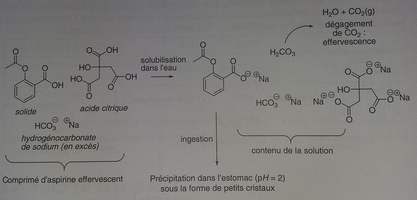
\includegraphics[scale = 0.75]{effervescence.png}
	\caption{Effervescence de l'aspirine.}
	\end{center}
\end{figure}

Le caractère bénéfique d'un principe actif est souvent fonction du dosage : "Rien n'est poison, tout est poison : seule la dose fait le poison", déclarait Paracelse au $\text{XV}^\text{e}$ siècle. C'est par exemple le cas de la \textbf{digitaline}, longtemps utilisée à faible dose comme cardiotonique pour le traitement de l'insuffisance cardiaque, mais qui à forte dose devient un poison très toxique, de même que le paracétamol.\\ 

Lorsqu'on synthétise un médicament, il est donc nécessaire de savoir doser les mélanges et de purifier les produits obtenus lors des synthèses, tout en appliquant la meilleure stratégie possible.\\

Nous allons maintenant réaliser la synthèse du principe actif de l'aspirine, l'acide acétylsalicylique. 

\newpage
\section{Synthèse et caractérisation de l'aspirine}\label{sec:2}

L'écorce de saule est utilisée depuis l'Antiquité égyptienne pour ses propriétés curatives, notamment pour soulager les douleurs et les fièvres. Le principe actif des décoctions de saule, la \textbf{salicyline} a été isolée par Leroux en 1829 et transformée en \textbf{acide salicylique} par Piria en 1838 par une hydrolyse (conduisant à l'alcool salicylique et au glucose) suivie d'une oxydation ménagée (chaîne carbonée préservée) par le dioxygène de l'air. Le rendement est mauvais.\\

C'est en 1860 que Kolbe permet une production industrielle en découvrant une synthèse de l'acide salicylique à partir du phénol (par carboxylation). En 1897, Hoffman met au point la synthèse de l'\textbf{acide acétylsalicylique}, brevetée sous le nom d'\textbf{Aspirine} par les laboratoires Bayer en 1899.

\begin{figure}[h!]
\begin{center}
	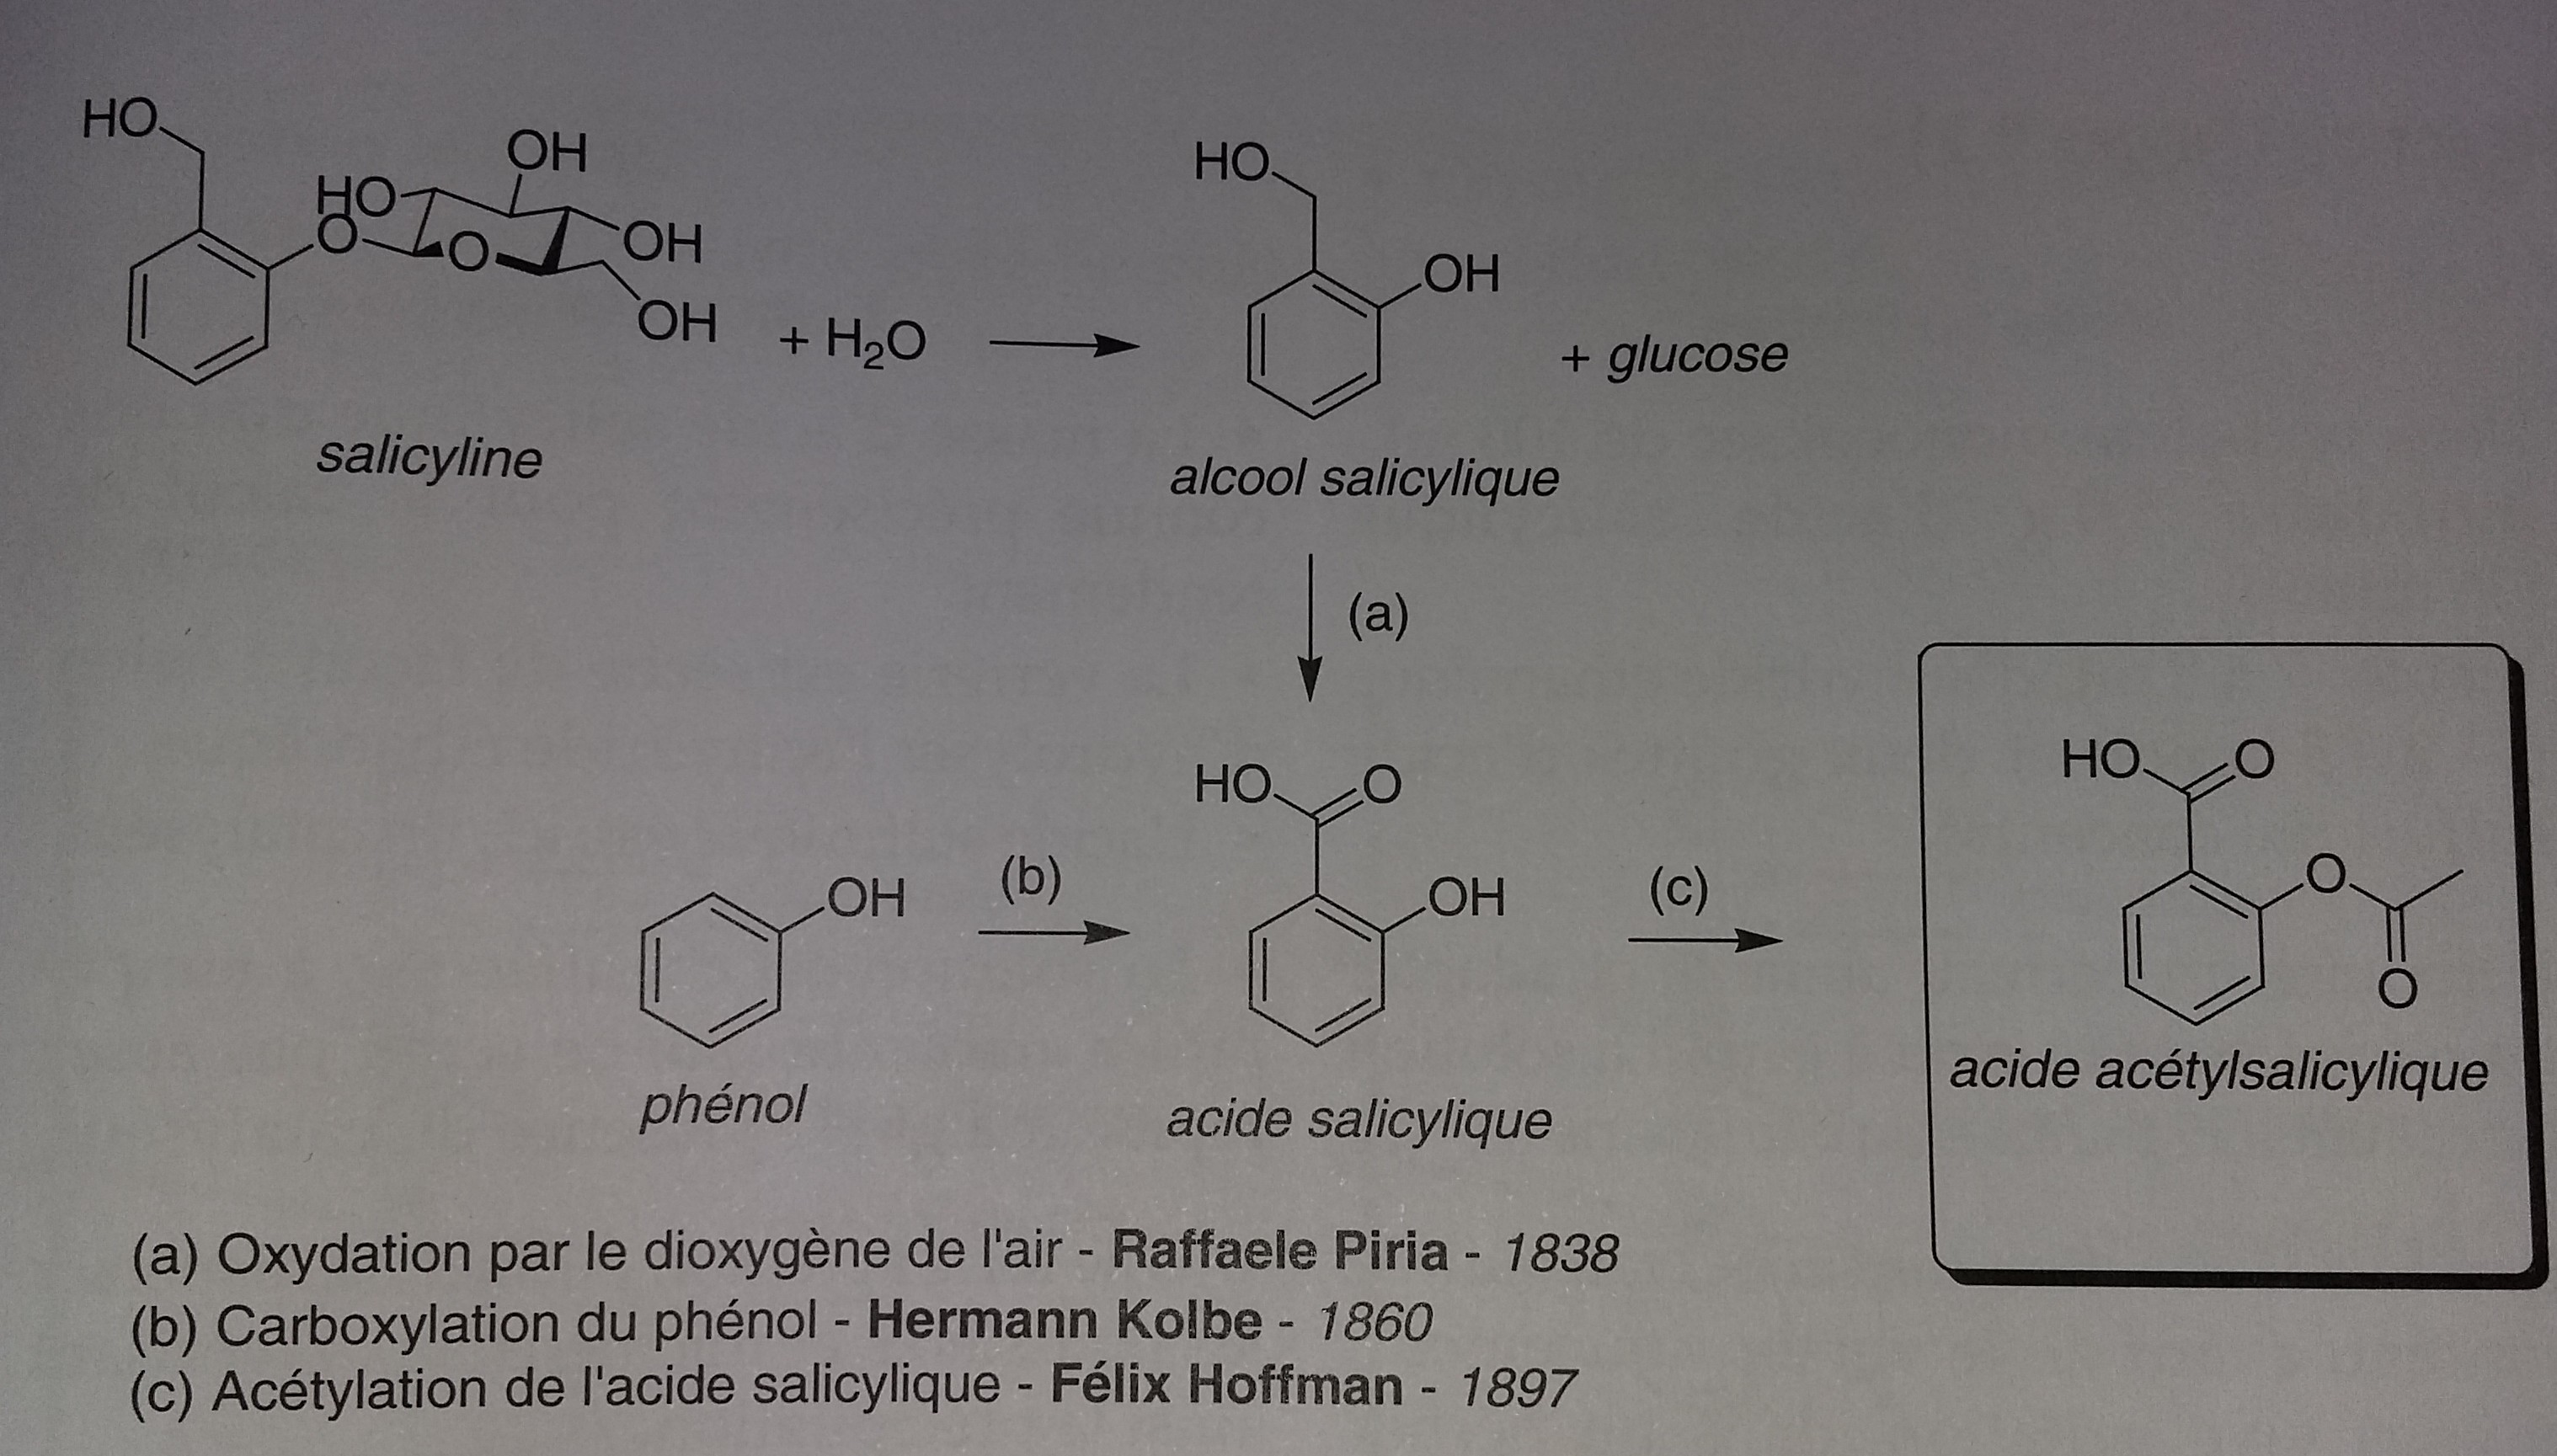
\includegraphics[scale = 0.1]{historique_aspirine.jpg}
	\caption{Historique de la synthèse de l'aspirine}. 
	\label{fig:historique}
\end{center}
\end{figure}

L'acide acétylsalicylique possède des propriétés : antalgiques (calme la douleur), antipyrétiques (calme la fièvre), anti-inflammatoires et anticoagulantes.

\subsection{Hémisynthèse de l'acide acétylsalicylique (Le Maréchal, tome 2, p149)}

Nous allons mettre en œuvre un protocole similaire à celui mis au point par Hoffmann. La réaction formant l'acide acétylsalicylique à partir de l'acide salicylique est une réaction d'\textbf{estérification} avec \textbf{l'acide acétique}, l'\textbf{acide salicylique jouant le rôle d'alcool} via sa fonction phénol.
\begin{figure}[h!]
\begin{center}
	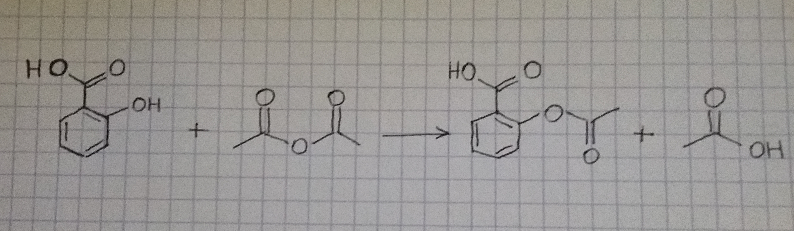
\includegraphics[scale = 0.3]{acetylation_acidesalicylique.png}
	\caption{Réaction de synthèse de l'aspirine à partir de l'anhydride éthanoïque}. 
	\label{fig:acetylation}
\end{center}
\end{figure}
Comme la réaction d'estérification est lente et équilibrée (rendement max 66\%), nous
utiliserons plutôt l'\textbf{anhydride acétique} (issu du dessèchement de deux acides éthanoïques) en catalyse acide (cf Figure \ref{fig:acetylation}) :
\begin{itemize}
	\item sa réactivité est plus grande que celle de l'acide éthanoïque, 
	et le catalyseur l'augmente encore;
	\item l'anhydride assèche le milieu réactionnel et empêche par conséquent l'hydrolyse de l'ester (réaction inverse de l'estérification), ce qui implique que la réaction d'estérification soit totale, la réaction inverse étant bloquée faute de réactif (l'eau);
	\item l'anhydride est introduit en excès : il sert de solvant.
\end{itemize}

\textbf{Instructions simplifiées}
\begin{itemize}
	\item \textcolor{red}{Faire deux synthèses en préparation : une complète avec recristallisation pour rendement, une autre sans recristallisation pour faire la filtration en direct. Expliquer le protocole, donner les quantités utilisées.}
	\item \textbf{Diviser par deux les quantités} indiquées sur le livre.
	\item Montage de chauffage à reflux contenant (précision requise) 2.5 g d'acide salicylique, 			4 mL d'anhydride éthanoïque (peser, pas de pipette car ce produit organique est pur) et 2 			gouttes d'acide sulfurique concentré (catalyseur).
	\item Dès que les réactifs sont en contact, mettre en marche l'agitation pour éviter la 				précipitation.
	\item Chauffer à 70$\degree$C (bain-marie) pendant 15 minutes en agitant.
	\item On refroidit le contenu puis on le verse sous vive agitation dans un bécher 
	contenant 30g de mélange eau glace. L'acide acétylsalicylique est peu soluble à froid, il va 		donc précipiter (solide blanc). Pas trop d'eau, et bien froide, sinon la réaction risque de 		repartir dans le sens indirect.\\
	
	\item \textbf{Données de la réaction :}\\
	\begin{center}
		\begin{tabular}{|c|c|c|}
 		\hline
  			Espèce & {Masse molaire} $\text{g}.\text{mol}^{-1}$ & Densité\\
  		\hline
  		\hline
  			Acide salicylique & 138.1 &\\
  		\hline 
  			Anhydride éthanoïque & 102.1 & 1.09\\
  		\hline
  			Acide acétylsalicylique & 180.2 &\\
  		\hline
   			Acide éthanoïque & 60.1 &\\
  		\hline
		\end{tabular}
	\end{center}
\end{itemize}

\begin{center}
	\begin{tabular}{cc}
  		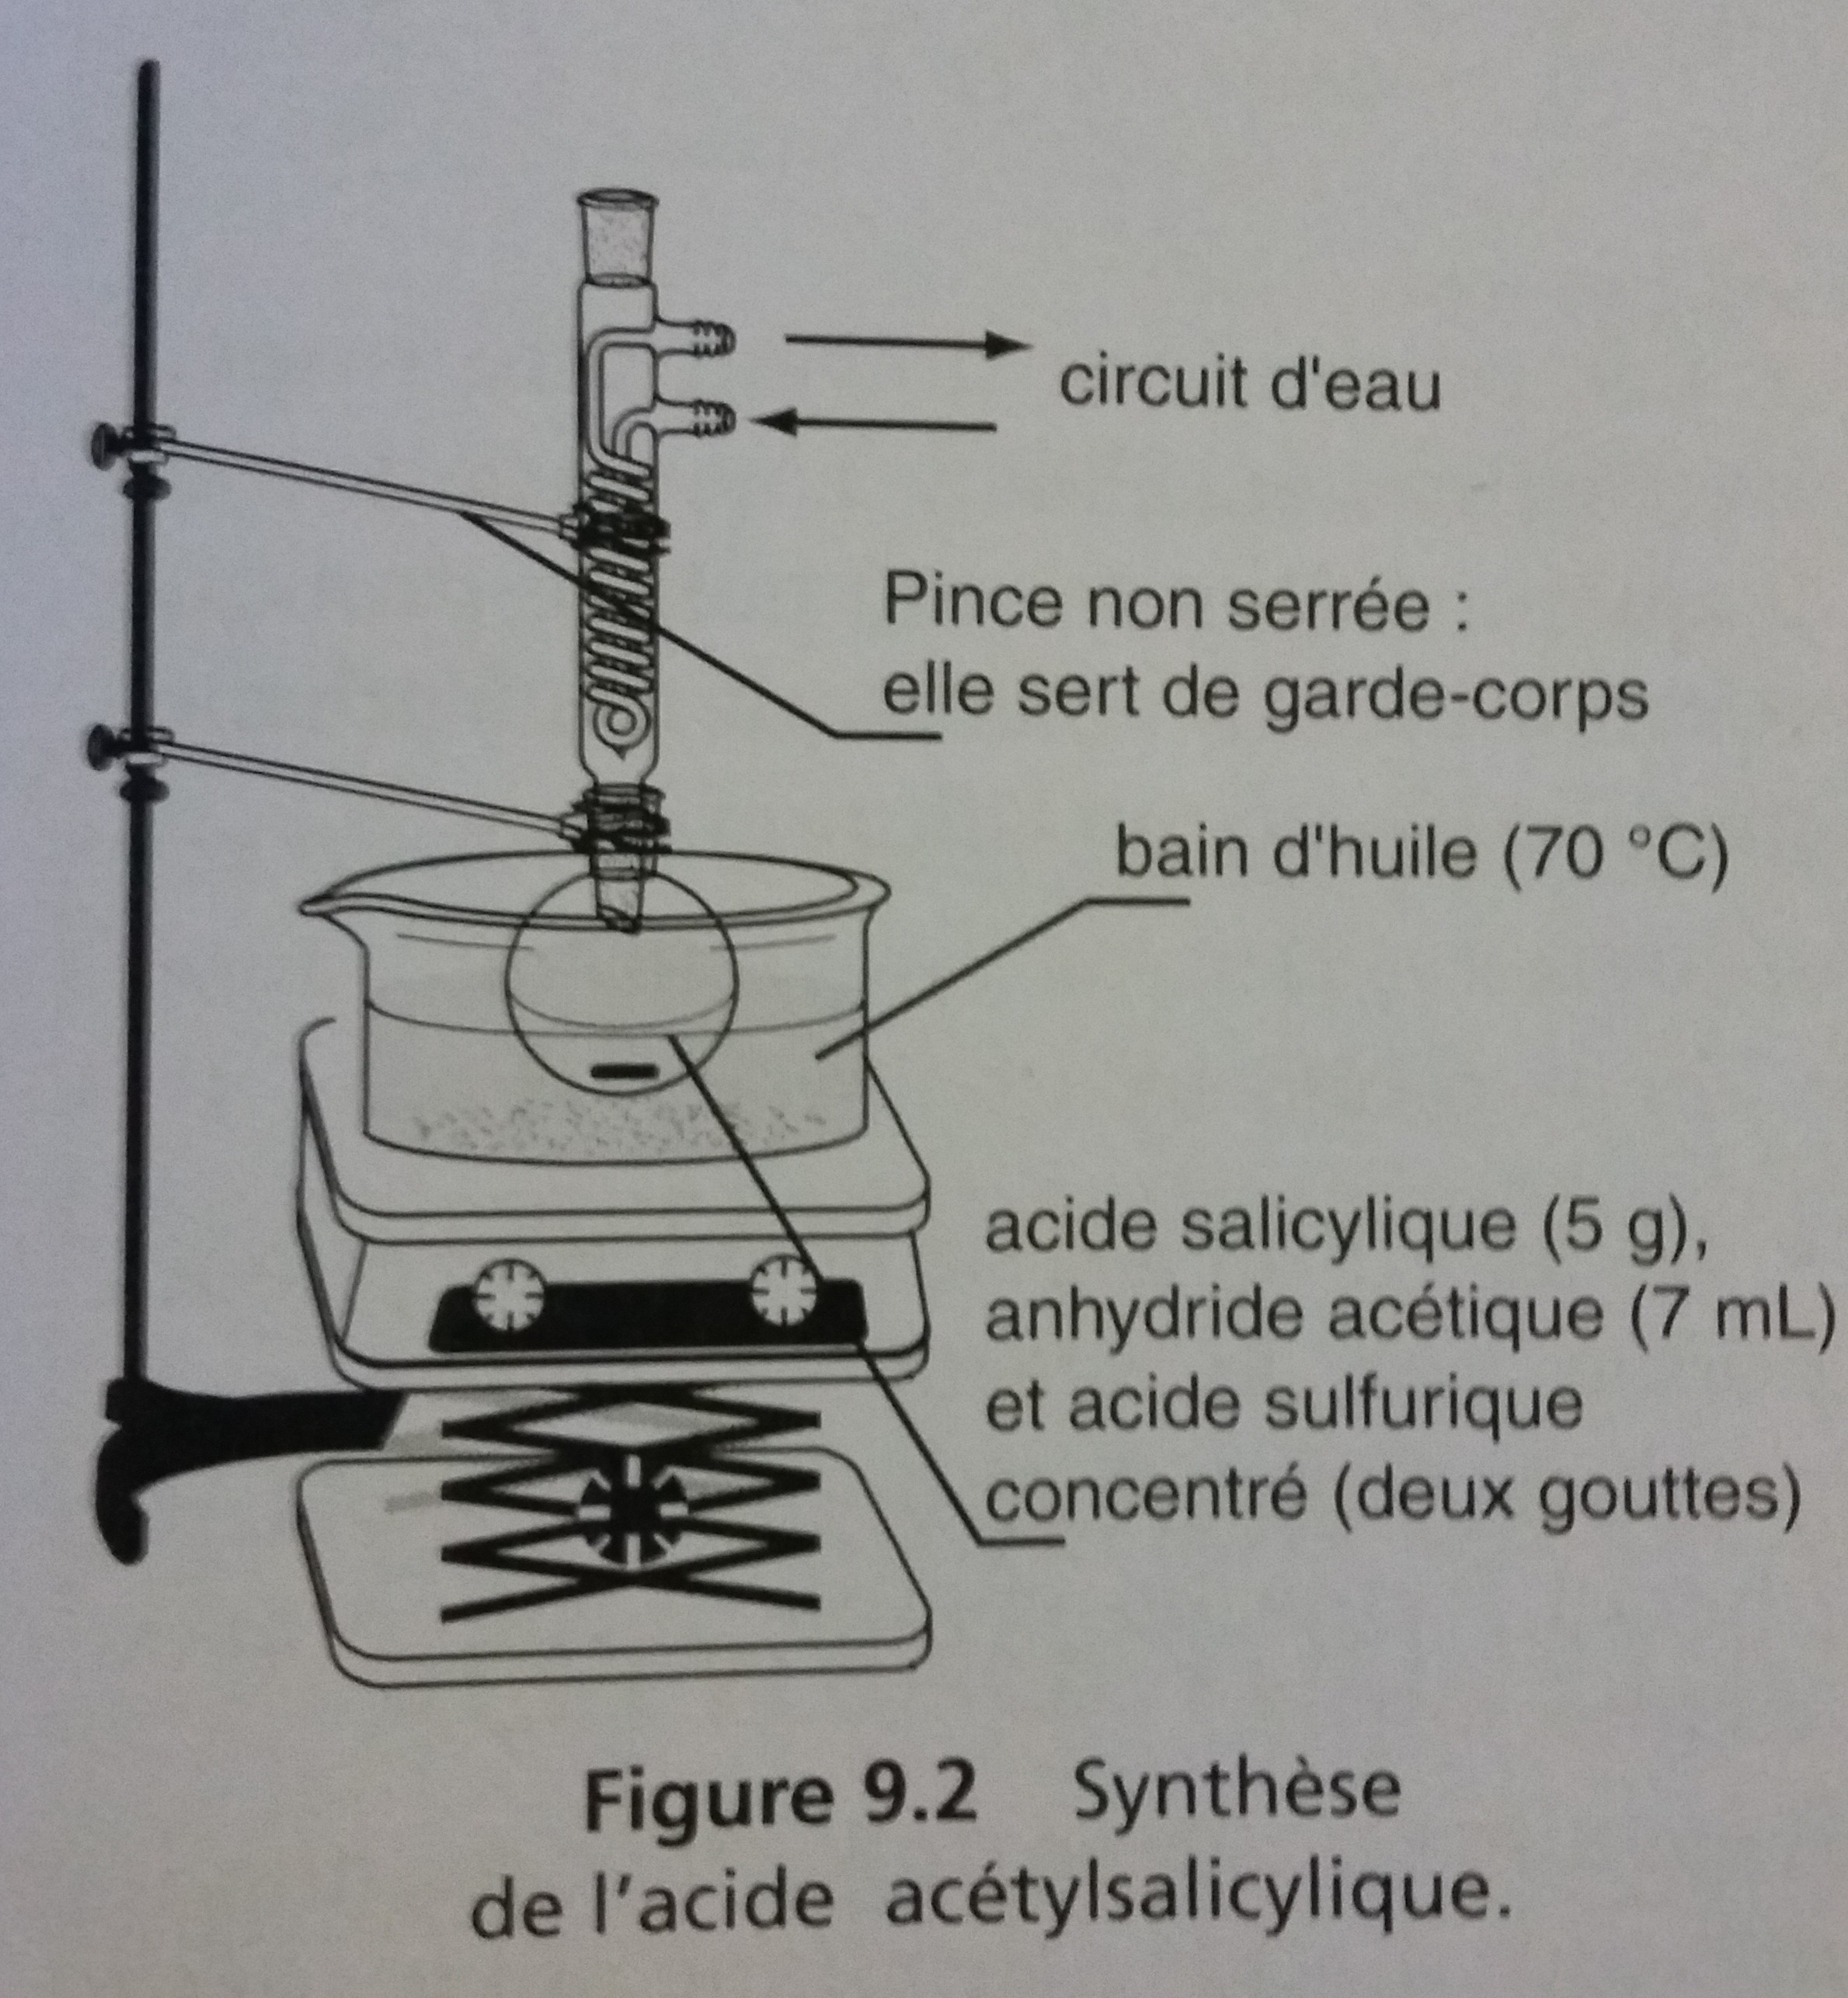
\includegraphics[scale = 0.1]{synthese_schema.jpg} &
   		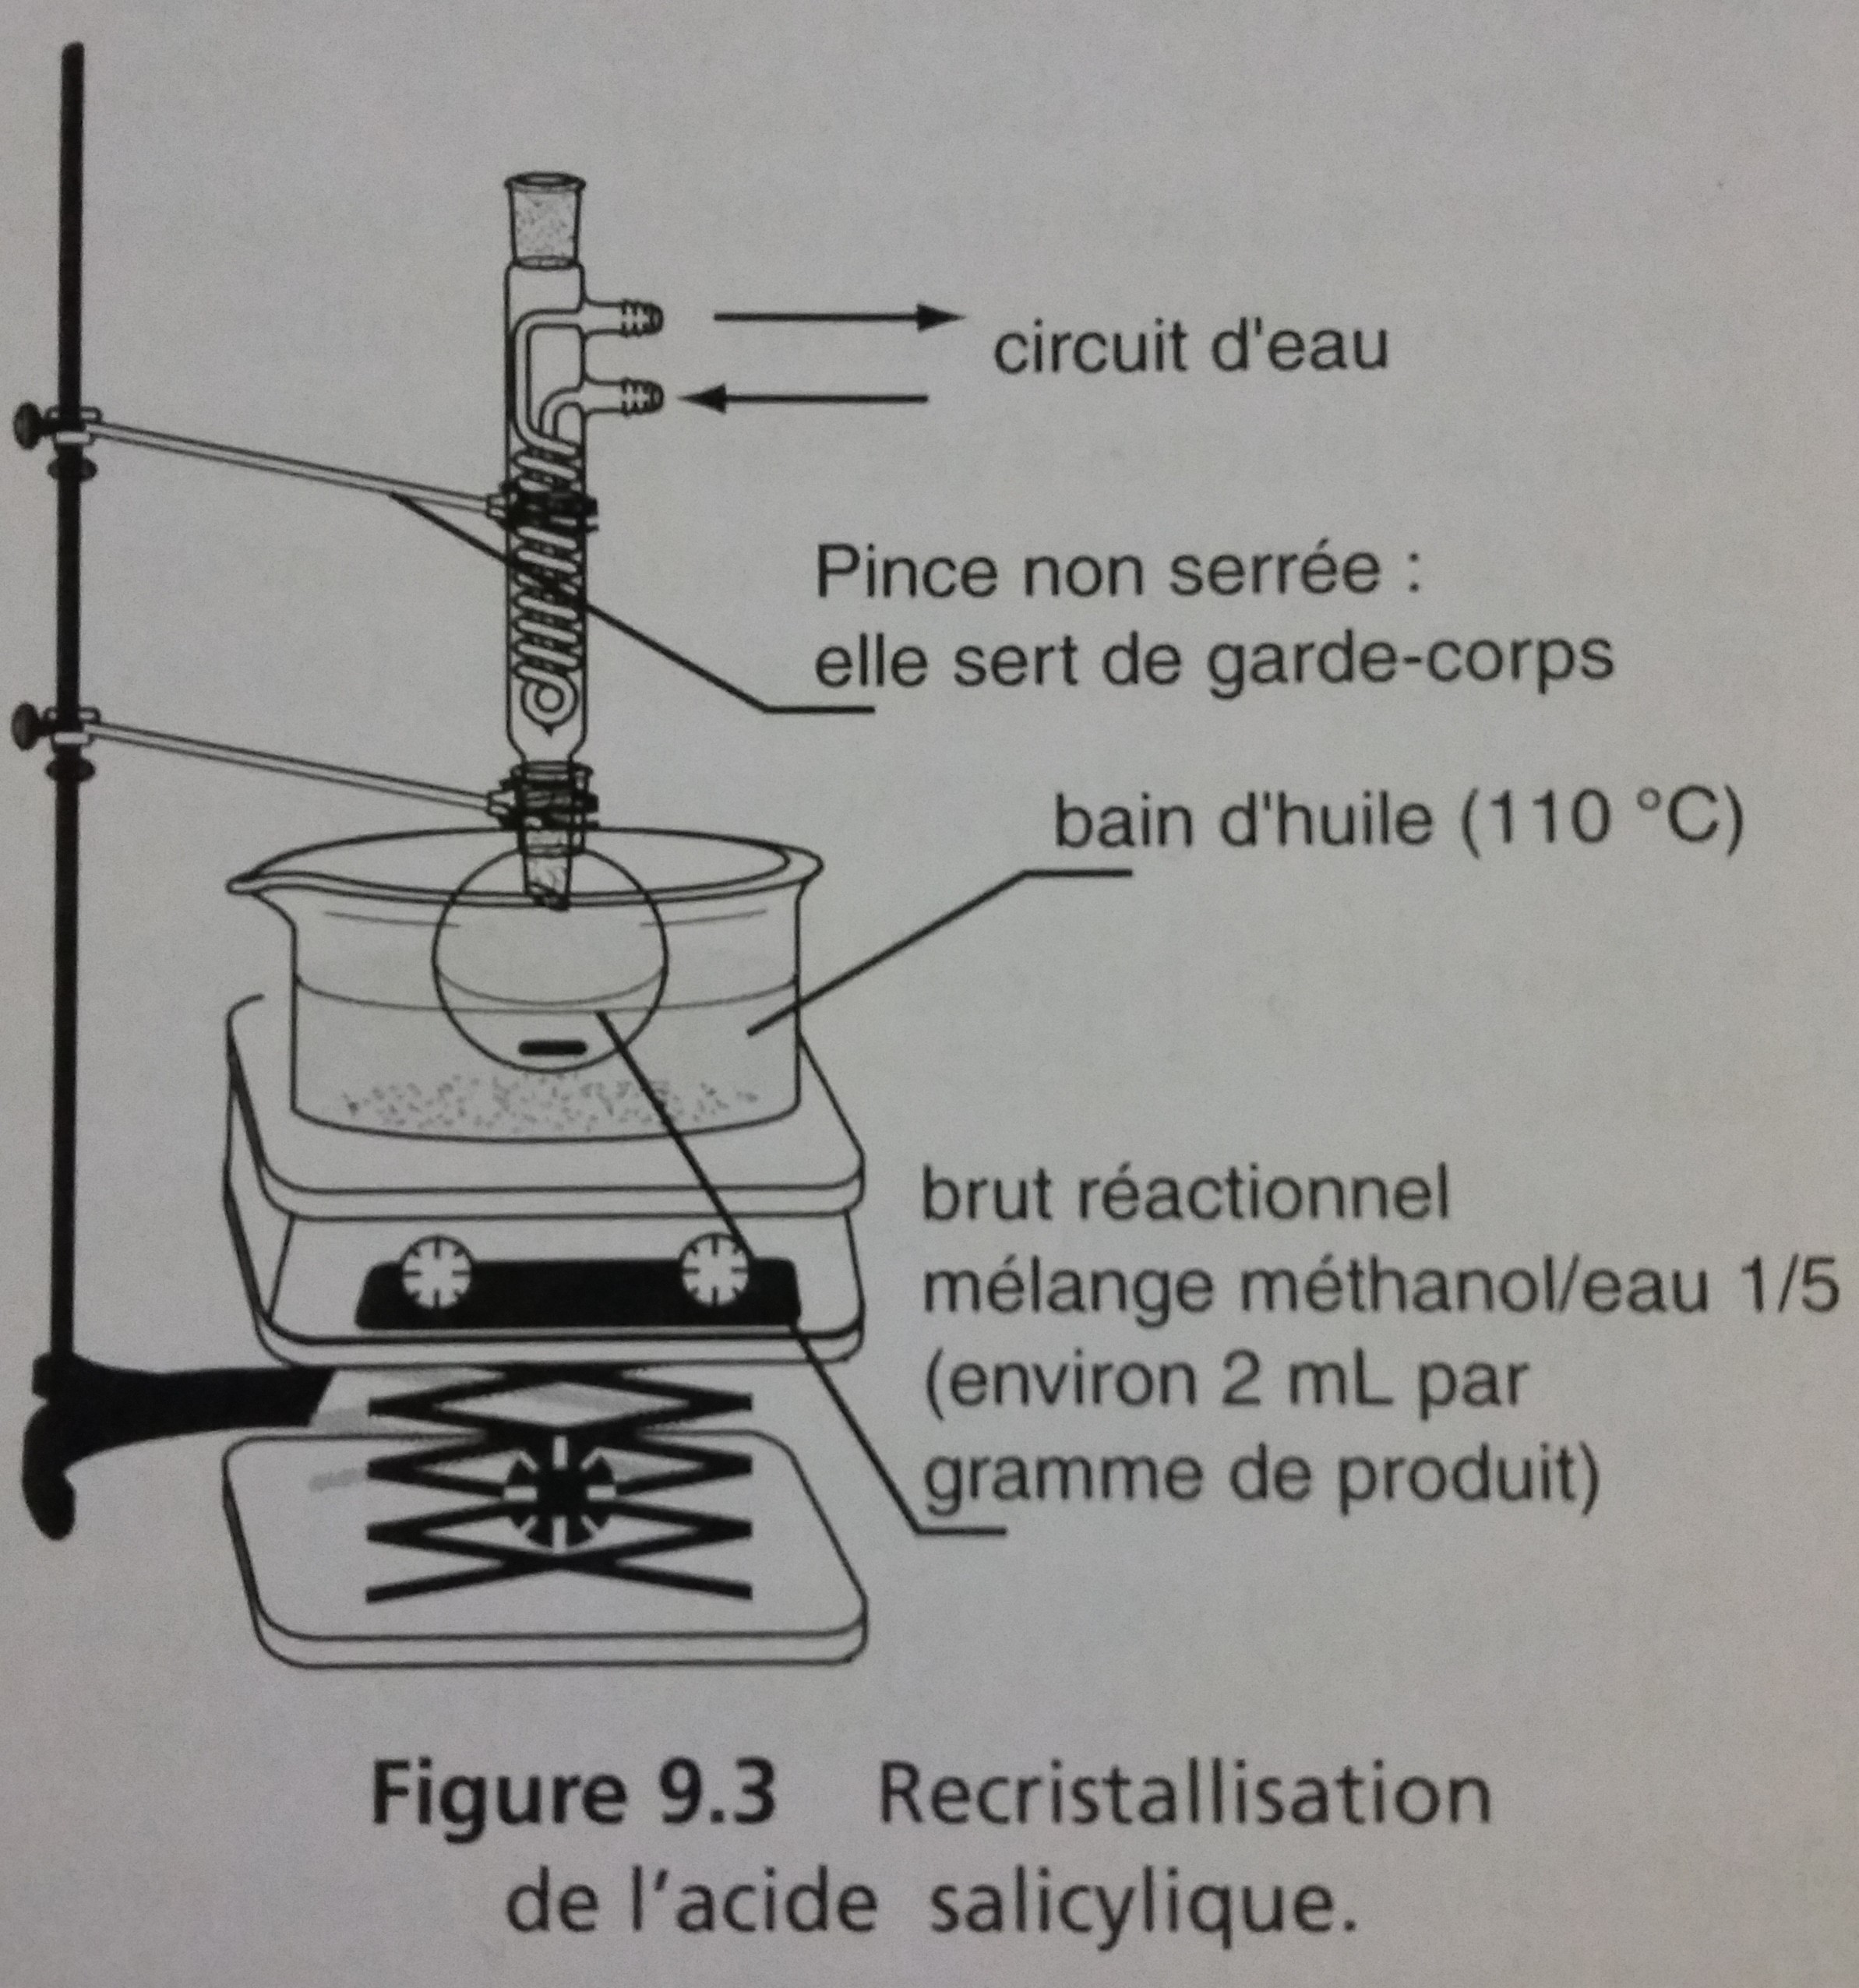
\includegraphics[scale = 0.1]{recristallisation_schema.jpg} \\
	\end{tabular}
\end{center}


\subsection{Purification par recristallisation (préparation)}

On récupère le précipité issu de la synthèse : il contient à la fois l'acide acétylsalicylique mais aussi de l'acide salicylique. \textbf{Il est important de purifier un médicament, d'où la recristallisation} pour éliminer l'acide salicylique :
\begin{itemize}
	\item $1/$ \textbf{Penser à conserver un petit échantillon de l'acide impur pour la suite}.
	\item $2/$ Filtrer le solide sur Büchner (le triturer d'abord avec une baguette de verre, 					avant d'activer l'aspiration, sans déchirer le papier filtre), rincer à l'eau froide. 				Le filtrat contient de l'eau et de l'acide éthanoïque (l'ajout d'eau permet aussi 					d'éliminer l'anhydride restant, il se change en acide). Le précipité solide contient 				le produit (acide acétylsalicylique) et l'acide salicylique n'ayant pas réagi.\\
\end{itemize}

Pour purifier le solide obtenu (éliminer l'acide salicylique piégé au milieu de l'acide acétylsalicylique), les deux espèces chimiques ayant des propriétés de solubilité voisines \textcolor{red}{à froid} on met en œuvre un procédé de recristallisation.\\

La recristallisation est une technique de base pour purifier les solides. Elle repose sur la différence de solubilité entre le composé à purifier et ses impuretés dans le solvant choisi. Par hypothèse, nous supposerons que les impuretés sont en concentration bien plus faible que le produit à purifier. La solubilité d'un composé augmente généralement avec la température.
Ainsi, on dissout le composé à purifier dans le minimum de solvant porté à ébullition. Par refroidissement, la solution se sature en composé à purifier mais les impuretés restent dissoutes.\\

\textbf{Protocole :}
\begin{itemize}
	\item Porter un mélange de solvants éthanol/eau en proportion 1/5 à ébullition. 15 mL 						suffisent.
	\item Dissoudre le brut réactionnel dans le mélange. 
	\item Si on peut filtrer en maintenant la température, filtrer à chaud : on élimine 						d'éventuelles impuretés, sinon passer à l'étape suivante.				).
	\item Laisser refroidir jusqu'à température ambiante. Les impuretés ne sont plus en assez 					grande quantité pour cristalliser.
	\item Filtrer à froid (filtration en direct) : les dernières impuretés partent dans le 						filtrat.
	\item Sécher à l'étuve.
	\item Peser le produit purifié et séché pour calculer le rendement.
\end{itemize}

\subsubsection{Rendement de la réaction}

Faire un tableau d'avancement (en direct).

\begin{equation}
	\boxed{\eta = \frac{\xi_f}{\xi_\text{max}}} = \frac{m_\text{produit}}{M_\text{produit}}\times 
	\frac{M_\text{réactif}}{m_\text{réactif}}
\end{equation}

L'acide acétylsalicylique est un acide faible ($\text{pKa} = 3.5$), que l'on pourrait doser avec une base forte, par exemple l'hydroxyde de sodium.

\subsection{Caractérisation de l'acide acétylsalicylique}

On veut s'assurer d'avoir synthétisé le bon produit ainsi que de sa pureté.

\subsubsection{Banc Köfler (indispensable et rapide)}

Le réactif et le produits ont des points de fusion différents. Un test au banc Köfler peut nous aider à confirmer la nature du produit obtenu. On doit le nettoyer avec un coton imbibé d'éthanol de la zone chaude à la zone froide. On étalonne avec un composé ayant une température de fusion entre $130\degree$ C et $140\degree$C.\\

\begin{itemize}
	\item Point de fusion de l'acide acétylsalicylique : $138\degree$ C. 
	\item Point de fusion de l'acide salicylique : $158\degree$ C.\\
\end{itemize}

\subsubsection{Test de la fonction phénol (facultatif)}

Le réactif porte une fonction phénol que ne possède plus le produit. Cette différence peut nous aider à évaluer la réussite du procédé de recristallisation et la pureté du produit recristallisé. Pour cela on prend trois tubes à essais dans lesquels on introduit :
\begin{itemize}
	\item Tube 1 : acide salicylique pur
	\item Tube 2 : produit avant recristallisation
	\item Tube 3 : acide acétylsalicylique recristallisé
	\item Éventuellement un tube 4 contenant du phénol.\\
\end{itemize}

Introduire \textbf{1 mL d'éthanol} (solvant pour dissoudre l'acide) et quelques \textbf{gouttes de chlorure de fer(III) à 1\% en masse} dans chaque tube. On constate, si tout va bien, l'apparition d'une couleur \textbf{violette dans les tubes 1 et 2} alors que le \textbf{tube 3 reste incolore}.\\

Interprétation : la fonction phénol, grâce au groupe hydroxyle, peut former un complexe coloré avec les ions fer(III), ce que ne peut pas faire l'acide acétylsalicylique.

\begin{figure}[h!]
\begin{center}
	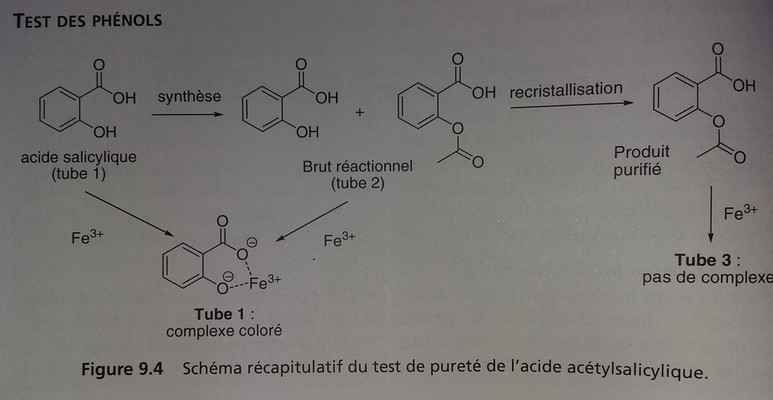
\includegraphics[scale = 0.5]{test_phenol.jpg}
	\label{fig:test_phenol}
\end{center}
\end{figure}

\subsubsection{Chromatographie sur couche mince}

On veut s'assurer de la pureté de notre produit : pour cela, on va faire une CCM (voir le Maréchal pour la commposition de l'éluant). Faire un dépôt test avec l'acide acétylsalicylique pur, un second avec l'acide salicylique pur, un troisième avec le produit non recristallisé et un quatrième avec le produit fini. Révélation à l'UV.

\subsubsection{Identification par spectroscopie IR}

Voir annexe pour les spectres.

\section{Antiseptiques, désinfectants, antibiotiques}

\subsection{Définitions}

Les \textbf{antiseptiques} sont des produits destinés à inhiber la croissance ou à tuer les micro-organismes et les virus au niveau de tissus vivants (peau saine, muqueuses, plaies). Ce sont donc des substances ayant une activité antibactérienne, antifongique, antivirale. Leurs conditions d’utilisation sont prévues pour ne pas altérer les tissus sur lesquels elles sont placées.\\

Les \textbf{désinfectants} ont également pour but de limiter la croissance ou de tuer les micro-organismes. Mais contrairement aux antiseptiques qui sont appliqués sur des tissus vivants, les désinfectants sont utilisés sur des matériaux inertes (sol, meubles, matériel médical).\\

Enfin, les \textbf{antibiotiques} sont des molécules capables de tuer des bactéries (effet bactéricide) ou d'inhiber leur croissance (effet bactériostatique) sans affecter les cellules de l'hôte. La plupart des antibiotiques actuels sont issus de molécules produites naturellement par des micro-organismes, et modifiées chimiquement pour améliorer leur activité et/ou changer certains paramètres. Par rapport aux antiseptiques et aux désinfectants, qui agissent généralement sur tous types de micro-organismes, les antibiotiques n'agissent que sur les bactéries, avec une spécificité \textbf{spectre} plus ou moins importante.

\begin{figure}[h!]
\begin{center}
	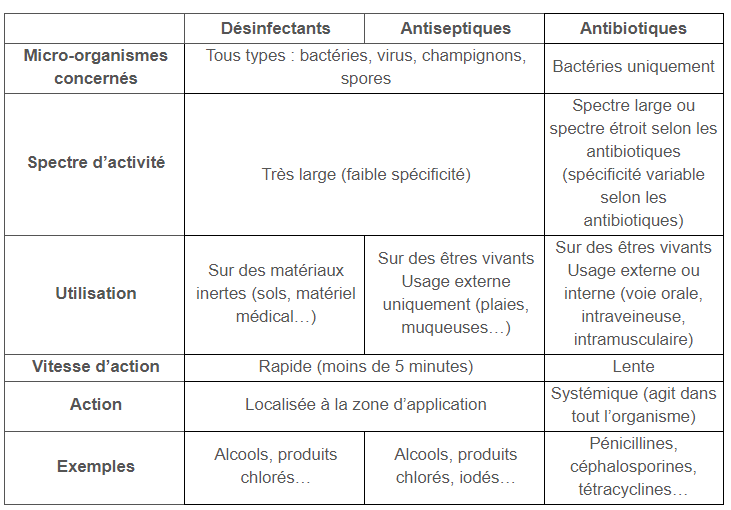
\includegraphics[scale = 0.8]{antis.png}
	\label{fig:antis}
\end{center}
\end{figure}

\subsection{Dosage du principe actif de la bétadine, le diiode (Cachau Redox, p299)}

La bétadine figure parmi les antiseptiques les plus connus. Elle est par exemple utilisée pour le lavage des mains oule nettoyage des plaies et l'antisepsie avant opération. Le principe actif de la bétadine est l'iode (ion triiodure). Dans la bétadine cet iode est lié à un polymère (la povidone) avec lequel elle forme un complexe. L'iode agit en oxydant les composés présents à l'intérieur des cellules ce qui, selon la dose employée, limite leur croissance ou les tue.

\begin{itemize}
	\item Ne pas diluer la bétadine. Thiosulfate de sodium à $10^{-2}$ mol/L.
\end{itemize}

\begin{figure}[h!]
\begin{center}
	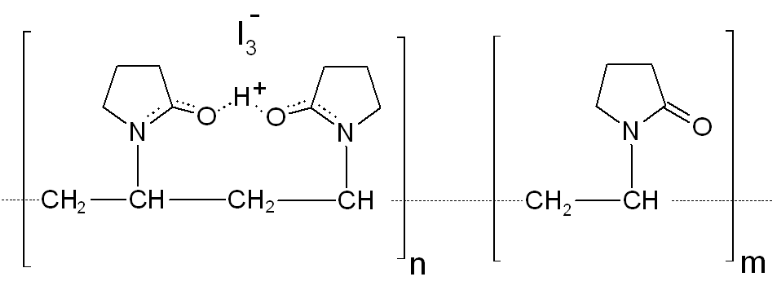
\includegraphics[scale = 0.5]{betadine.png}
	\label{fig:betadine}
\end{center}
\end{figure}

\textcolor{red}{La povidone a un effet tensioactif lorsqu'on introduit vivement de l'eau dans la bétadine, ce qui produit de la mousse. Il faut donc faire attention lors du dosage (et éviter de diluer la bétadine). Le pourcentage massique indiqué sur le flacon de bétadine tient compte de la masse de la povidone. Comme c'est un polymère, on ne peut que connaître une masse molaire moyenne et non exacte : ce pourcentage est donc inutilisable pour analyser un dosage. On fait confiance à la concentration en diiode indiquée sur le Cachau (mais on ne dilue pas la bétadine comme le livre le conseille, sous peine de se retrouver avec de la mousse et surtout un volume équivalent trop faible).}\\

\textbf{Couples rédox en présence :} $\text{I}_2/\text{I}^-$ (diiode, ion iodure), et 
$\text{S}_2\text{O}_4^{2-}/\text{S}_4\text{O}_6^{2-}$ (ion thiosulfate, ion tétrathionate).

\newpage
\section*{Conclusion}

Insister sur l'importance de la pureté des médicaments. Mentionner l'existence de trafics de médicaments frauduleux aux conséquences dramatiques. La synthèse des médicaments est de la chimie fine, qui implique souvent de nombreuses étapes, ce qui est difficile compatible avec les exigences de la chimie verte, d'où la recherche de nouveaux modes de synthèse pour réduire le gaspillage d'atomes et la production de déchets. Il existe d'autres types de médicaments : on pourrait par exemple mentionner les radionucléïdes, utilisés en imagerie médicale ou en radiothérapie. Ils sont considérés comme des médicaments, prescrits par un médecin et produits par un radiopharmacien.

\newpage
\section*{Annexes}
\subsection*{Mécanisme de la synthèse de l'acide acétylsalicylique}

\begin{figure}[h!]
\begin{center}
	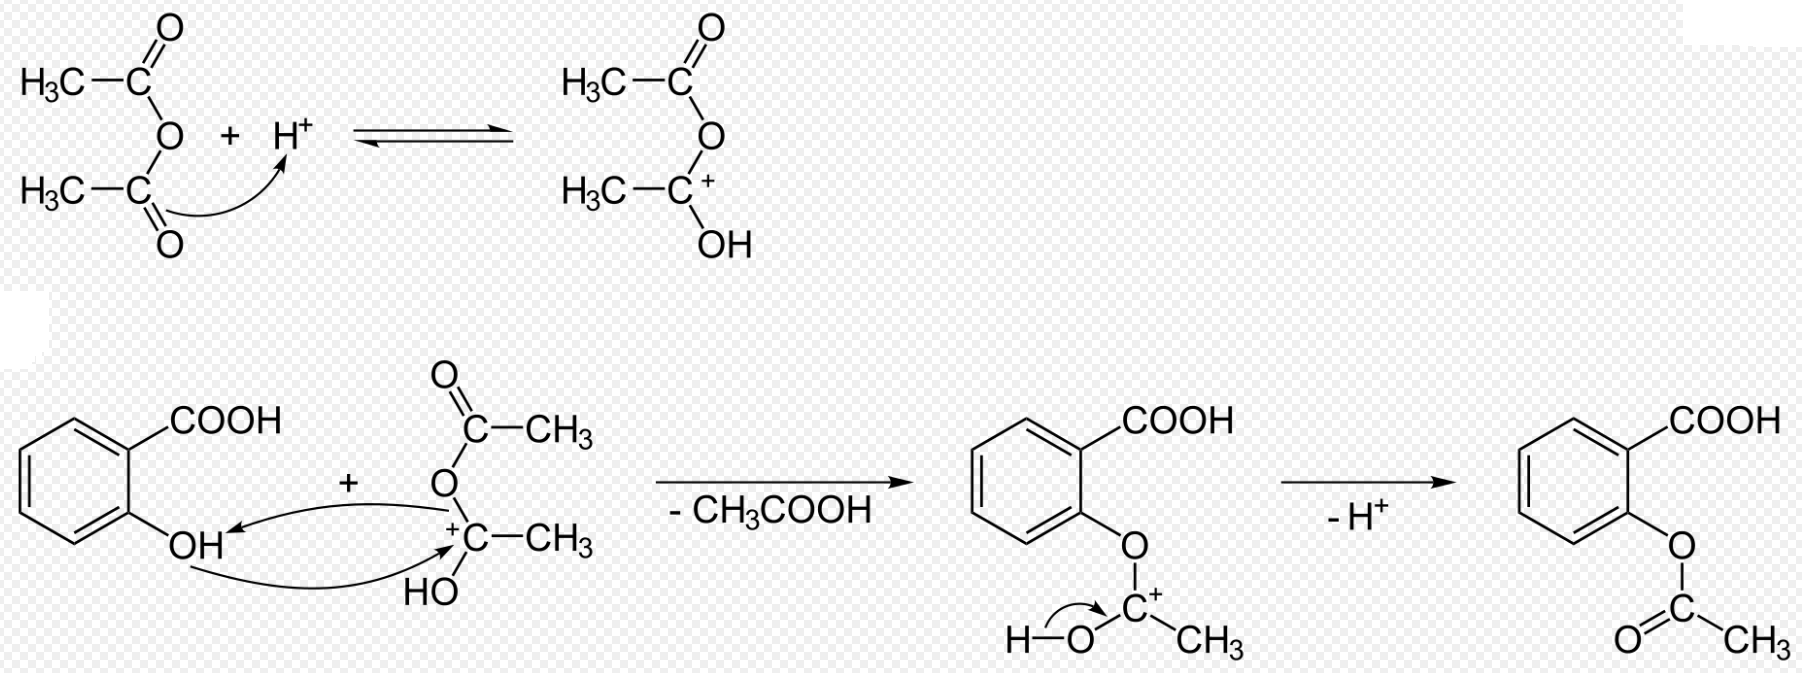
\includegraphics[scale = 0.35]{mecanisme_synth.png}
	\label{fig:mecanisme}
\end{center}
\end{figure}

\newpage
\subsection*{Spectres IR}

\begin{figure}[h!]
	\begin{center}
		\begin{tabular}{c}
  		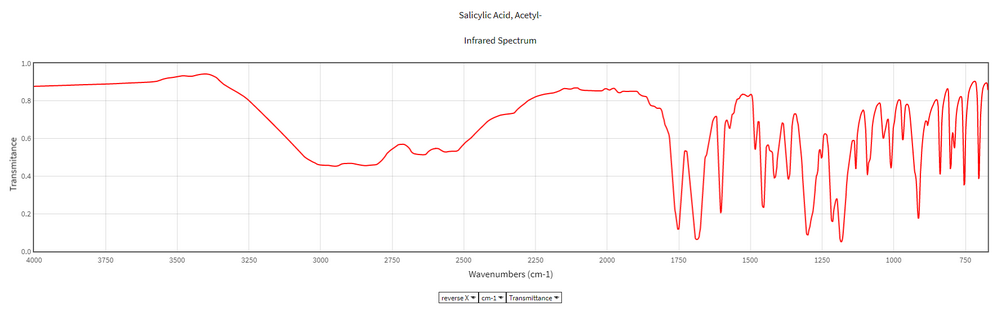
\includegraphics[scale = 0.6]{IR_aspirine.png} \\
   		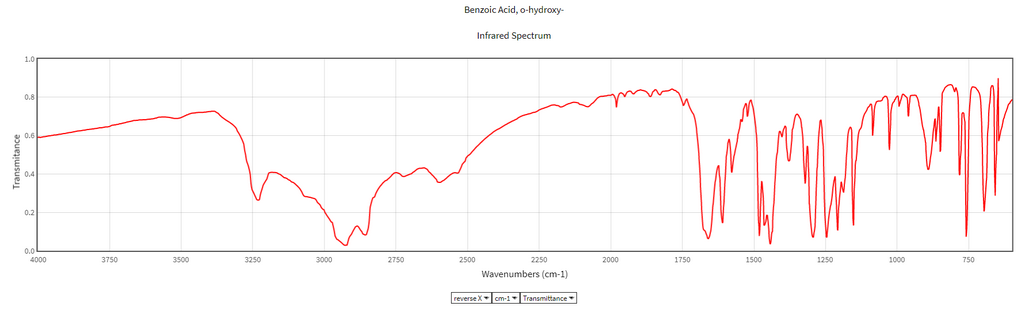
\includegraphics[scale = 0.6]{IR_acidesalicylique.png}\\
	    \end{tabular}
		\caption{Spectres IR de l'aspirine (haut) et de l'acide salicylique (bas).}
	\end{center}
\end{figure}
\end{document}